%%%%%%%%%%%%%%%%%%%%%%%%%%%%%%%%%%%%%%%%%%%%%%%%%%%%%%%%%%%%%%%%%%%%%%%%%%%%%%%%
%% Plantilla de memoria en LaTeX para la ETSIT - Universidad Rey Juan Carlos
%%
%% Por Gregorio Robles <grex arroba gsyc.urjc.es>
%%     Grupo de Sistemas y Comunicaciones
%%     Escuela Tcnica Superior de Ingenieros de Telecomunicacin
%%     Universidad Rey Juan Carlos
%% (muchas ideas tomadas de Internet, colegas del GSyC, antiguos alumnos...
%%  etc. Muchas gracias a todos)
%%
%% La ltima versin de esta plantilla est siempre disponible en:
%%     https://github.com/gregoriorobles/plantilla-memoria
%%
%% Para obtener PDF, ejecuta en la shell:
%%   make
%% (las imgenes deben ir en PNG o JPG)

%%%%%%%%%%%%%%%%%%%%%%%%%%%%%%%%%%%%%%%%%%%%%%%%%%%%%%%%%%%%%%%%%%%%%%%%%%%%%%%%

\documentclass[a4paper, 12pt]{book}
%\usepackage[T1]{fontenc}
\usepackage{hyperref}
\usepackage[a4paper, left=2.5cm, right=2.5cm, top=3cm, bottom=3cm]{geometry}
\usepackage{times}
\usepackage[latin1]{inputenc}
\usepackage[spanish,activeacute]{babel} % Comenta esta lnea si tu memoria es en ingls
\usepackage{url}
%\usepackage[dvipdfm]{graphicx}
\usepackage{fancybox}
\usepackage{subfigure}
\usepackage{graphicx}
\usepackage{float}  %% H para posicionar figuras
\usepackage[nottoc, notlot, notlof, notindex]{tocbibind} %% Opciones de ndice
\usepackage{latexsym}  %% Logo LaTeX

\title{Memoria del Proyecto}
\author{Adri\'an S\'aez Clemente}

\renewcommand{\baselinestretch}{1.5}  %% Interlineado

\begin{document}

%\renewcommand{\refname}{Bibliografa}  %% Renombrando
\renewcommand{\appendixname}{Ap\'endice}

%%%%%%%%%%%%%%%%%%%%%%%%%%%%%%%%%%%%%%%%%%%%%%%%%%%%%%%%%%%%%%%%%%%%%%%%%%%%%%%%
% PORTADA

\begin{titlepage}
\begin{center}
\begin{tabular}[c]{c c}
%\includegraphics[bb=0 0 194 352, scale=0.25]{logo} &

\includegraphics[scale=0.25]{img/logo_vect.png} &
\begin{tabular}[b]{l}
\Huge
\textsf{UNIVERSIDAD} \\
\Huge
\textsf{REY JUAN CARLOS} \\
\end{tabular}
\\
\end{tabular}

\vspace{3cm}

\Large
GRADO EN INGENIER\'IA EN TECNOLOG\'IAS DE LA TELECOMUNICACI\'ON

\vspace{0.4cm}

\large
Curso Acad\'emico 2014/2015

\vspace{0.8cm}

Trabajo Fin de Grado

\vspace{2.5cm}

\LARGE
DESARROLLO Y DESPLIEGUE DE APLICACIONES EN EL \'AMBITO EDUCATIVO

\vspace{4cm}

\large
Autor : Adri\'an S\'aez Clemente \\
Tutor : Gregorio Robles Mart\'inez
\end{center}
\end{titlepage}

\newpage
\mbox{}
\thispagestyle{empty} % para que no se numere esta pagina


%%%%%%%%%%%%%%%%%%%%%%%%%%%%%%%%%%%%%%%%%%%%%%%%%%%%%%%%%%%%%%%%%%%%%%%%%%%%%%%%
%%%% Dedicatoria

%\chapter*{}
%\pagenumbering{Roman} % para comenzar la numeracion de paginas en numeros romanos
%\begin{flushright}
%\textit{Dedicado a \\
%mi familia / mi abuelo / mi abuela}
%\end{flushright}

%%%%%%%%%%%%%%%%%%%%%%%%%%%%%%%%%%%%%%%%%%%%%%%%%%%%%%%%%%%%%%%%%%%%%%%%%%%%%%%%
%%%% Agradecimientos

\chapter*{Agradecimientos}
\addcontentsline{toc}{chapter}{Agradecimientos} % si queremos que aparezca en el ndice
\markboth{AGRADECIMIENTOS}{AGRADECIMIENTOS} % encabezado 

Aqu vienen los agradecimientos\ldots Aunque est bien acordarse de la pareja,
no hay que olvidarse de dar las gracias a tu madre, que aunque a veces no lo 
parezca disfrutar tanto de tus logros como t\ldots Adems, la pareja quizs
no sea para siempre, pero tu madre s.

%%%%%%%%%%%%%%%%%%%%%%%%%%%%%%%%%%%%%%%%%%%%%%%%%%%%%%%%%%%%%%%%%%%%%%%%%%%%%%%%
%%%% Resumen

\chapter*{Resumen}
\addcontentsline{toc}{chapter}{Resumen} % si queremos que aparezca en el ndice
\markboth{RESUMEN}{RESUMEN} % encabezado

En este proyecto se realiza el desarrollo de una aplicaci\'on web que se basa en la creaci\'on de una plataforma....

\begin{itemize}
  \item De qu va este proyecto? Cul es su objetivo principal?
  \item Cmo se ha realizado? Qu tecnologas estn involucradas?
  \item En qu contexto se ha realizado el proyecto? Es un proyecto
dentro de un marco general?
\end{itemize}

Lo mejor es escribir el resumen al final.

%%%%%%%%%%%%%%%%%%%%%%%%%%%%%%%%%%%%%%%%%%%%%%%%%%%%%%%%%%%%%%%%%%%%%%%%%%%%%%%%
%%%% Resumen en ingls

\chapter*{Summary}
\addcontentsline{toc}{chapter}{Summary} % si queremos que aparezca en el ndice
\markboth{SUMMARY}{SUMMARY} % encabezado

Here comes a translation of the ``Resumen'' into English. Please, double check
it for correct grammar and spelling. As it is the translation of the ``Resumen'',
which is supposed to be written at the end, this as well should be filled out
just before submitting.


%%%%%%%%%%%%%%%%%%%%%%%%%%%%%%%%%%%%%%%%%%%%%%%%%%%%%%%%%%%%%%%%%%%%%%%%%%%%%%%%
%%%%%%%%%%%%%%%%%%%%%%%%%%%%%%%%%%%%%%%%%%%%%%%%%%%%%%%%%%%%%%%%%%%%%%%%%%%%%%%%
% NDICES %
%%%%%%%%%%%%%%%%%%%%%%%%%%%%%%%%%%%%%%%%%%%%%%%%%%%%%%%%%%%%%%%%%%%%%%%%%%%%%%%%

% Las buenas noticias es que los ndices se generan automticamente.
% Lo nico que tienes que hacer es elegir cules quieren que se generen,
% y comentar/descomentar esa instruccin de LaTeX.

%%%% ndice de contenidos
\tableofcontents 
%%%% ndice de figuras
\cleardoublepage
\phantomsection
\addcontentsline{toc}{chapter}{Lista de figuras} % para que aparezca en el indice de contenidos
\listoffigures % indice de figuras
%%%% ndice de tablas
%\cleardoublepage
%\addcontentsline{toc}{chapter}{Lista de tablas} % para que aparezca en el indice de contenidos
%\listoftables % indice de tablas


%%%%%%%%%%%%%%%%%%%%%%%%%%%%%%%%%%%%%%%%%%%%%%%%%%%%%%%%%%%%%%%%%%%%%%%%%%%%%%%%
%%%%%%%%%%%%%%%%%%%%%%%%%%%%%%%%%%%%%%%%%%%%%%%%%%%%%%%%%%%%%%%%%%%%%%%%%%%%%%%%
% INTRODUCCIN %
%%%%%%%%%%%%%%%%%%%%%%%%%%%%%%%%%%%%%%%%%%%%%%%%%%%%%%%%%%%%%%%%%%%%%%%%%%%%%%%%

\cleardoublepage
\chapter{Introducci\'on}
\label{sec:intro} % etiqueta para poder referenciar luego en el texto con ~\ref{sec:intro}
\pagenumbering{arabic} % para empezar la numeracin de pgina con nmeros

\section{Descripci\'on del proyecto}
En este proyecto se implementa una aplicaci\'on web que consiste en el desarrollo de un planeta de blogs. Est\'a enfocado al \'ambito educativo y puede
ser usado en cualquier entorno que simule un aula, ya sea en universidades, institutos, colegios, academias, cursos online, etc,...

El contenido de la aplicaci\'on recoge autom\'aticamente mensajes o entradas de un conjunto de blogs que comparten una tem\'atica com\'un.

El tutor ser\'a el responsable de crear hilos donde los alumnos podr\'an suscribirse y formar parte de la tem\'atica de inter\'es. Dentro de cada hilo,
los alumnos podr\'an visualizar las entradas del conjunto de blogs que est\'an suscritos a ese hilo.

Como novedad incluye la posibilidad de interactuar, valorar y comentar los mensajes de compa\~neros de una forma divertida mediante un proceso de 
gamificaci\'on. En este proceso los participantes de cada hilo podr\'an luchar por un puesto en la clasificaci\'on definitiva consiguiendo 
puntos (llamados planets) y subiendo de nivel seg\'un el compromiso y la capacidad de interacci\'on de cada alumno.

Existe una secci\'on de b\'usqueda para poder encontrar entradas introduciendo nick de usuario y/o identificador de entrada. Y adem\'as, dentro de la
aplicaci\'on se puede encontrar otra secci\'on con las bases de las puntuaciones.

\section{Contexto tecnol\'ogico}


\section{}
\label{sec:}

\subsection{Estilo}
\label{subsec:estilo}

Sobre el uso de las comas\footnote{\url{http://narrativabreve.com/2015/02/opiniones-de-un-corrector-de-estilo-11-recetas-para-escribir-correctamente-la-coma.html}}

 \begin{figure}
    \centering
    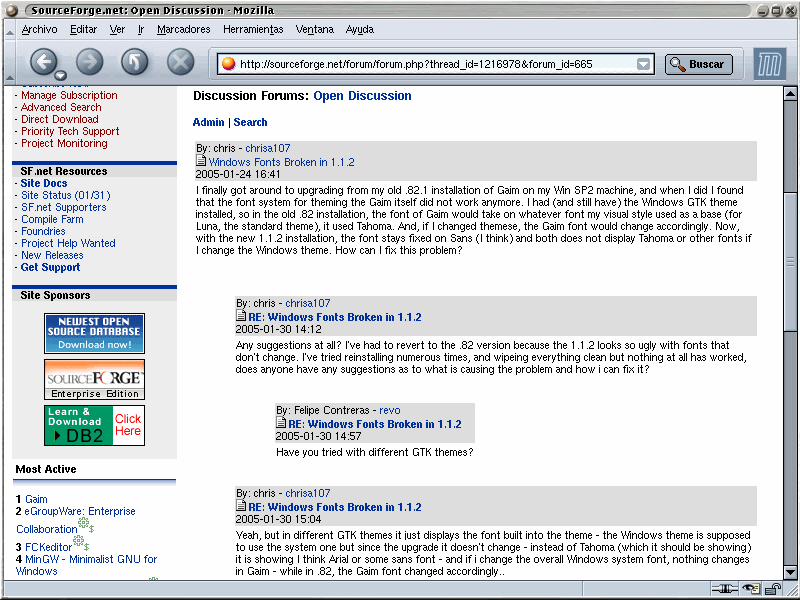
\includegraphics[bb=0 0 800 600, width=12cm, keepaspectratio]{img/foro1}
    \caption{Pgina con enlaces a hilos}
    \label{figura:foro_hilos}
 \end{figure}

{\footnotesize
\begin{verbatim}
    From gaurav at gold-solutions.co.uk  Fri Jan 14 14:51:11 2005
    From: gaurav at gold-solutions.co.uk (gaurav_gold)
    Date: Fri Jan 14 19:25:51 2005
    Subject: [Mailman-Users] mailman issues
    Message-ID: <003c01c4fa40$1d99b4c0$94592252@gaurav7klgnyif>

    Dear Sir/Madam,
    How can people reply to the mailing list?  How do i turn off
    this feature? How can i also enable a feature where if someone
    replies the newsletter the email gets deleted?
    Thanks

    From msapiro at value.net  Fri Jan 14 19:48:51 2005
    From: msapiro at value.net (Mark Sapiro)
    Date: Fri Jan 14 19:49:04 2005
    Subject: [Mailman-Users] mailman issues
    In-Reply-To: <003c01c4fa40$1d99b4c0$94592252@gaurav7klgnyif>
    Message-ID: <PC173020050114104851057801b04d55@msapiro>

    gaurav_gold wrote:
    >How can people reply to the mailing list?  How do i turn off
    this feature? How can i also enable a feature where if someone
    replies the newsletter the email gets deleted?

    See the FAQ
    >Mailman FAQ: http://www.python.org/cgi-bin/faqw-mm.py
    article 3.11
\end{verbatim}
}




%%%%%%%%%%%%%%%%%%%%%%%%%%%%%%%%%%%%%%%%%%%%%%%%%%%%%%%%%%%%%%%%%%%%%%%%%%%%%%%%
%%%%%%%%%%%%%%%%%%%%%%%%%%%%%%%%%%%%%%%%%%%%%%%%%%%%%%%%%%%%%%%%%%%%%%%%%%%%%%%%
% OBJETIVOS %
%%%%%%%%%%%%%%%%%%%%%%%%%%%%%%%%%%%%%%%%%%%%%%%%%%%%%%%%%%%%%%%%%%%%%%%%%%%%%%%%

\cleardoublepage
\chapter{Objetivos}
\label{chap:objetivos}

\section{Objetivo general}
label{sec:objetivo-general}


\section{Objetivos especficos}
label{sec:objetivos-especificos}


\section{Planificacin temporal}
label{sec:planificacion-temporal}



%%%%%%%%%%%%%%%%%%%%%%%%%%%%%%%%%%%%%%%%%%%%%%%%%%%%%%%%%%%%%%%%%%%%%%%%%%%%%%%%
%%%%%%%%%%%%%%%%%%%%%%%%%%%%%%%%%%%%%%%%%%%%%%%%%%%%%%%%%%%%%%%%%%%%%%%%%%%%%%%%
% ESTADO DEL ARTE %
%%%%%%%%%%%%%%%%%%%%%%%%%%%%%%%%%%%%%%%%%%%%%%%%%%%%%%%%%%%%%%%%%%%%%%%%%%%%%%%%

\cleardoublepage
\chapter{Estado del arte}

Descripcin de las tecnologas que utilizas en tu trabajo. Con dos o tres prrafos por cada tecnologa, vale.


Puedes citar libros, como el de Bonabeau et al. sobre procesos estigmrgicos~\cite{bonabeau:_swarm}. % Nota que el ~ aade un espacio en blanco, pero no deja que exista un salto de lnea. Imprescindible ponerlo para las citas.

Tambin existe la posibilidad de poner notas al pie de pgina, por ejemplo, 
una para indicarte que visite la pgina de 
LibreSoft\footnote{\url{http://www.libresoft.es}}.

\section{Seccin 1} 
\label{sec:seccion1}



%%%%%%%%%%%%%%%%%%%%%%%%%%%%%%%%%%%%%%%%%%%%%%%%%%%%%%%%%%%%%%%%%%%%%%%%%%%%%%%%
%%%%%%%%%%%%%%%%%%%%%%%%%%%%%%%%%%%%%%%%%%%%%%%%%%%%%%%%%%%%%%%%%%%%%%%%%%%%%%%%
% DISEO E IMPLEMENTACIN %
%%%%%%%%%%%%%%%%%%%%%%%%%%%%%%%%%%%%%%%%%%%%%%%%%%%%%%%%%%%%%%%%%%%%%%%%%%%%%%%%

\cleardoublepage
\chapter{Diseo e implementacin}

\section{Arquitectura general} 
\label{sec:arquitectura}

figura~\ref{fig:arquitectura}.

\begin{figure}
  \centering
  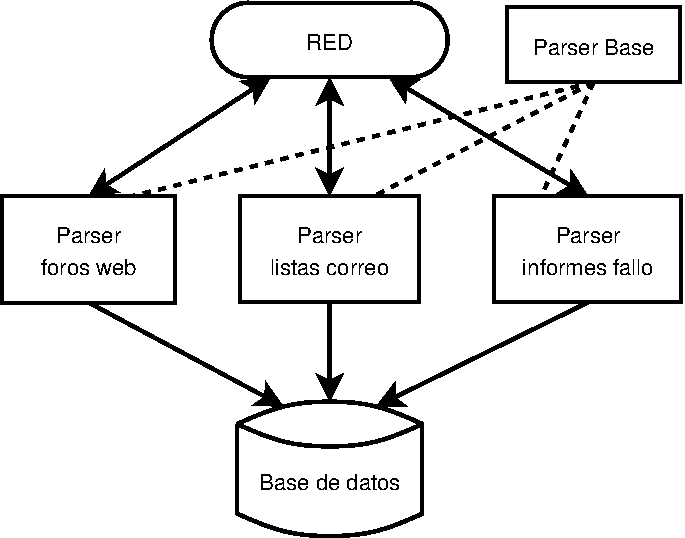
\includegraphics[width=9cm, keepaspectratio]{img/arquitectura}
  \caption{Estructura del parser bsico}
  \label{fig:arquitectura}
\end{figure}



%%%%%%%%%%%%%%%%%%%%%%%%%%%%%%%%%%%%%%%%%%%%%%%%%%%%%%%%%%%%%%%%%%%%%%%%%%%%%%%%
%%%%%%%%%%%%%%%%%%%%%%%%%%%%%%%%%%%%%%%%%%%%%%%%%%%%%%%%%%%%%%%%%%%%%%%%%%%%%%%%
% RESULTADOS %
%%%%%%%%%%%%%%%%%%%%%%%%%%%%%%%%%%%%%%%%%%%%%%%%%%%%%%%%%%%%%%%%%%%%%%%%%%%%%%%%

\cleardoublepage
\chapter{Resultados}




%%%%%%%%%%%%%%%%%%%%%%%%%%%%%%%%%%%%%%%%%%%%%%%%%%%%%%%%%%%%%%%%%%%%%%%%%%%%%%%%
%%%%%%%%%%%%%%%%%%%%%%%%%%%%%%%%%%%%%%%%%%%%%%%%%%%%%%%%%%%%%%%%%%%%%%%%%%%%%%%%
% CONCLUSIONES %
%%%%%%%%%%%%%%%%%%%%%%%%%%%%%%%%%%%%%%%%%%%%%%%%%%%%%%%%%%%%%%%%%%%%%%%%%%%%%%%%

\cleardoublepage
\chapter{Conclusiones}
\label{chap:conclusiones}


\section{Consecucin de objetivos}
\label{sec:consecucion-objetivos}

Esta seccin es la seccin espejo de las dos primeras del captulo de objetivos,
donde se planteaba el objetivo general y se elaboraban los especficos.

Es aqu donde hay que debatir qu se ha conseguido y qu no. Cuando algo no
se ha conseguido, se ha de justificar, en trminos de qu problemas se han
encontrado y qu medidas se han tomado para mitigar esos problemas.


\section{Aplicacin de lo aprendido}
\label{sec:aplicacion}

Aqu viene lo que has aprendido durante el Grado/Mster y que has aplicado
en el TFG/TFM. Una buena idea es poner las asignaturas ms relacionadas y
comentar en un prrafo los conocimientos y habilidades puestos en prctica.

\begin{enumerate}
  \item a
  \item b
\end{enumerate}


\section{Lecciones aprendidas}
\label{sec:lecciones_aprendidas}

Aqu viene lo que has aprendido en el Trabajo Fin de Grado/Mster.

\begin{enumerate}
  \item a
  \item b
\end{enumerate}


\section{Trabajos futuros}
\label{sec:trabajos_futuros}

Ningn software se termina, as que aqu vienen ideas y funcionalidades
que estara bien tener implementadas en el futuro.

Es un apartado que sirve para dar ideas de cara a futuros TFGs/TFMs.


\section{Valoracin personal}
\label{sec:valoracion}

Finalmente (y de manera opcional), hay gente que se anima a dar su punto de
vista sobre el proyecto, lo que ha aprendido, lo que le gustara haber aprendido,
las tecnologas utilizadas y dems.



%%%%%%%%%%%%%%%%%%%%%%%%%%%%%%%%%%%%%%%%%%%%%%%%%%%%%%%%%%%%%%%%%%%%%%%%%%%%%%%%
%%%%%%%%%%%%%%%%%%%%%%%%%%%%%%%%%%%%%%%%%%%%%%%%%%%%%%%%%%%%%%%%%%%%%%%%%%%%%%%%
% APNDICE(S) %
%%%%%%%%%%%%%%%%%%%%%%%%%%%%%%%%%%%%%%%%%%%%%%%%%%%%%%%%%%%%%%%%%%%%%%%%%%%%%%%%

\cleardoublepage
\appendix
\chapter{Manual de usuario}
\label{app:manual}

\section{P\'agina de inicio}
\begin{figure}[htbp] 
  \label{figura:inicio}
  \centering
  \shadowbox{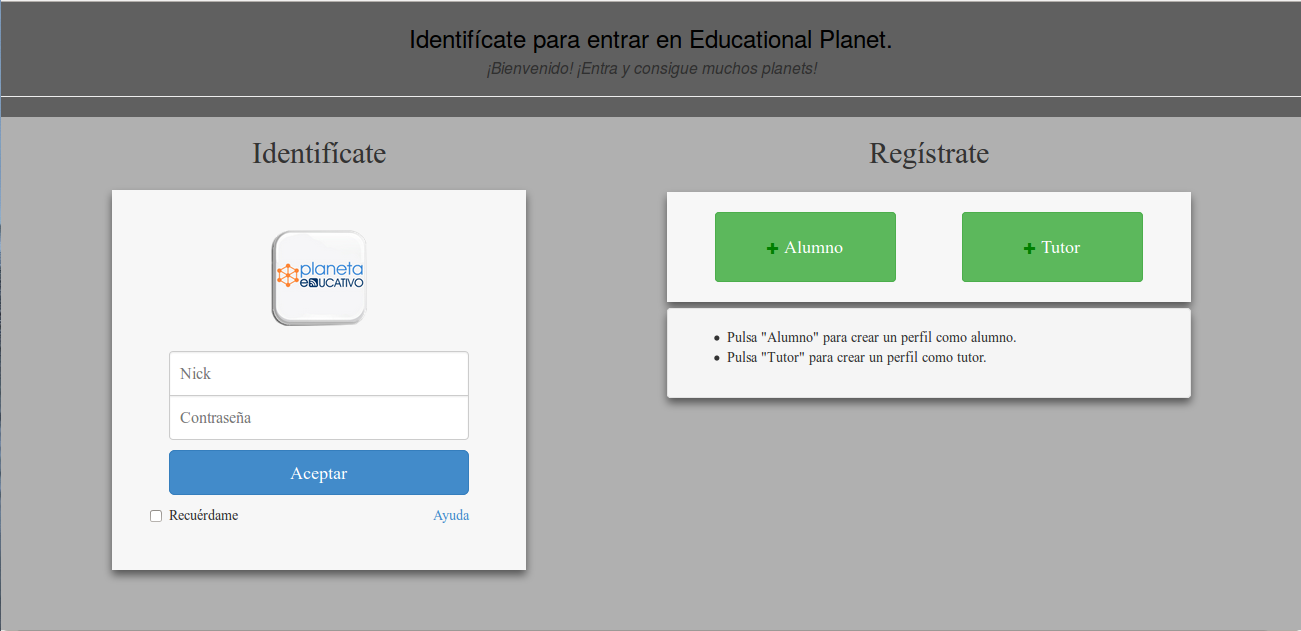
\includegraphics[width=17cm, keepaspectratio]{imagenes/PaginaInicio}}
  \caption{P\'agina de inicio}
\end{figure}
\begin{figure}[htbp] 
  \label{figura:inicio1}
  \centering
  \subfigure[Inicio de sesi\'on]{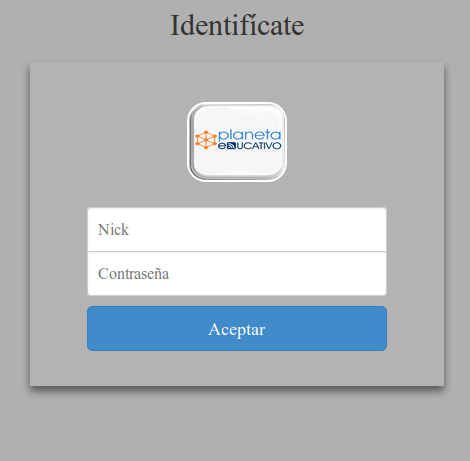
\includegraphics[width=6cm]{imagenes/InicioComoAlumno}}
  \subfigure[Inicio de sesi\'on err\'onea]{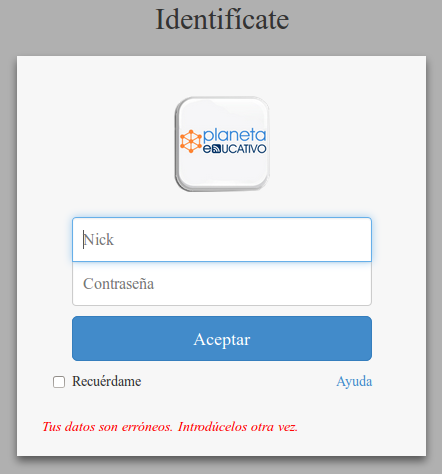
\includegraphics[width=6cm]{imagenes/InicioError}}
  \caption{Inicio de sesi\'on}
\end{figure}
\newpage
\paragraph{}
Como se muestra en la figura


\newpage
\section{P\'agina de registro}
\begin{figure}[htbp] 
  \label{figura:registro}
  \centering
  \shadowbox{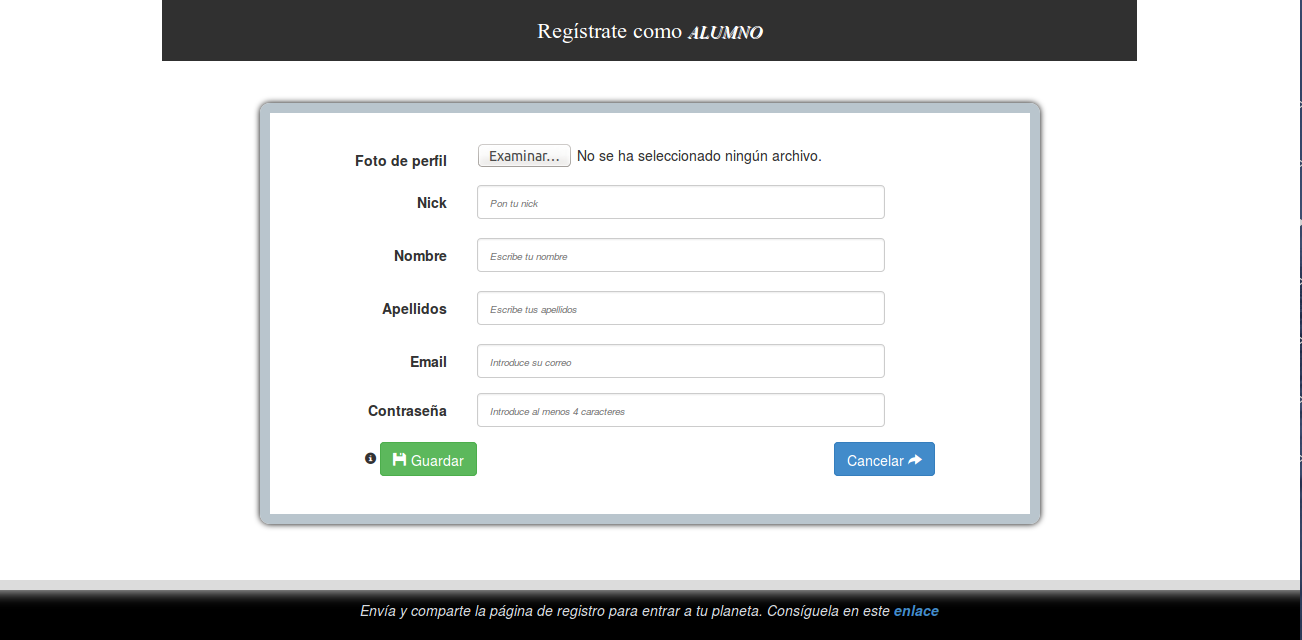
\includegraphics[width=17cm, keepaspectratio]{imagenes/RegistroAlumno}}
  \caption{Registro como alumno}
\end{figure}
\begin{figure}[htbp] 
  \label{figura:registro1}
  \centering
  \shadowbox{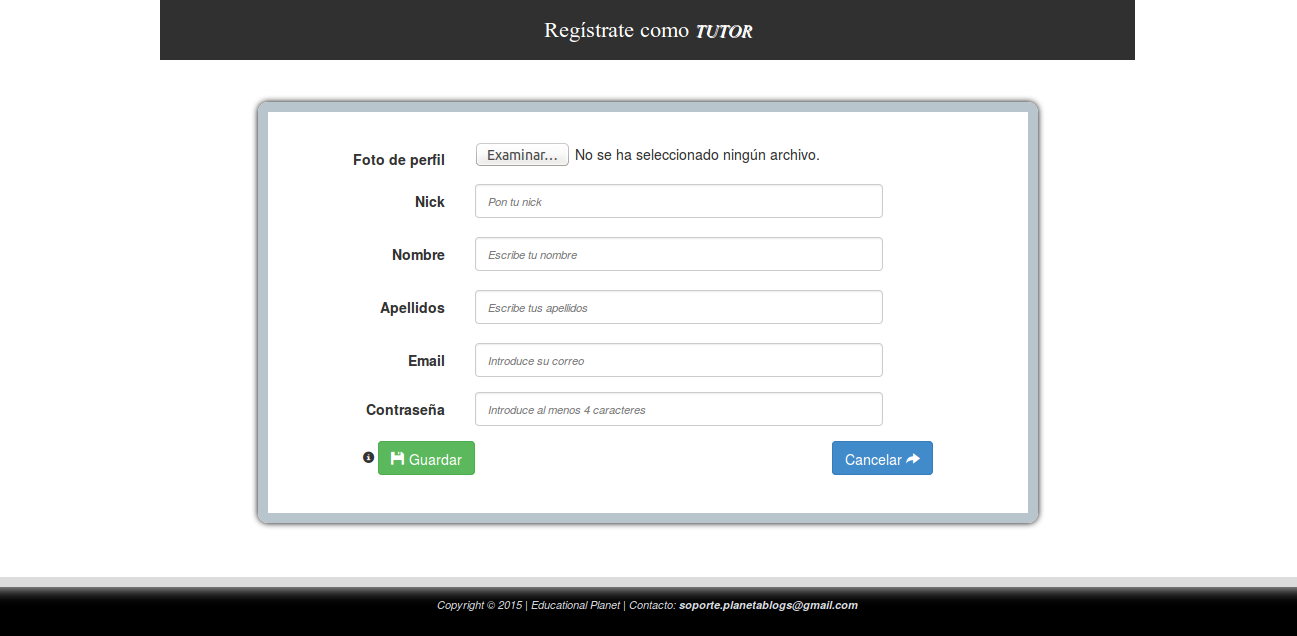
\includegraphics[width=17cm, keepaspectratio]{imagenes/RegistroTutor}}
  \caption{Registro como tutor}
\end{figure}
\begin{figure}[htbp] 
  \label{figura:registro2}
  \centering
  \shadowbox{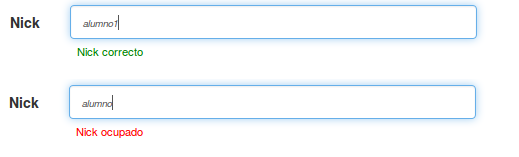
\includegraphics[width=17cm, keepaspectratio]{imagenes/NickCorrectoOcupado}}
  \caption{Rellenar nick}
\end{figure}
\begin{figure}[htbp] 
  \label{figura:registro3}
  \centering
  \shadowbox{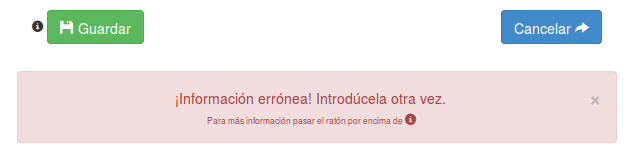
\includegraphics[width=17cm, keepaspectratio]{imagenes/RegistroAlumnoError}}
  \caption{Registro err\'oneo}
\end{figure}
\begin{figure}[htbp] 
  \label{figura:registro4}
  \centering
  \shadowbox{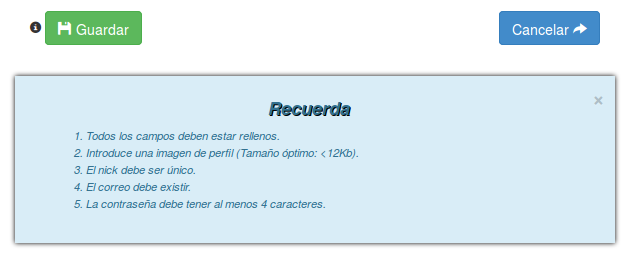
\includegraphics[width=17cm, keepaspectratio]{imagenes/RegistroAlumnoInfo}}
  \caption{Informaci\'on de registro}
\end{figure}
se muestra todo

\newpage
\section{Presentaci\'on de tutor}
\begin{figure}[htbp] 
  \label{figura:tutor}
  \centering
  \shadowbox{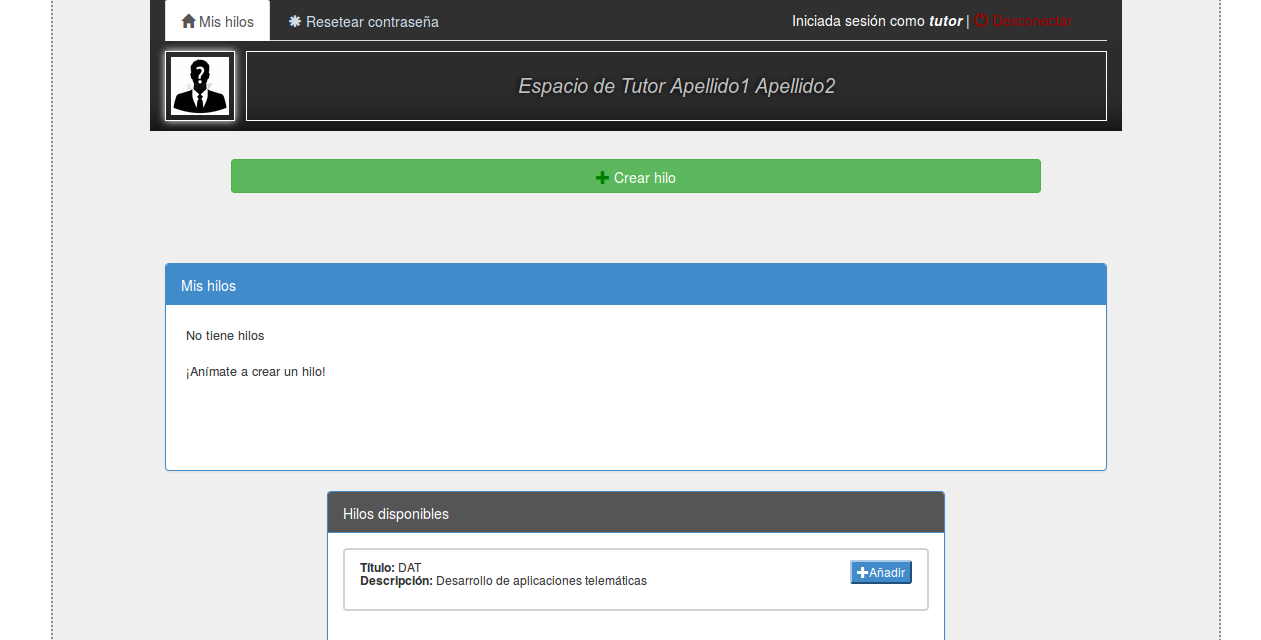
\includegraphics[width=17cm, keepaspectratio]{imagenes/PresentacionTutor}}
  \caption{P\'agina de presentaci\'on de tutor}
\end{figure}
figura \hyperref[figura:registro1]{A.4}
\newpage
%%%%%%%%%%%%%%%%%%%%%%%%%%%%%%%%%%%%%%%%%%%%%%%%%%%%%%%%%%%%%%%%%%%%%%%%%%%%%%%%
%%%%%%%%%%%%%%%%%%%%%%%%%%%%%%%%%%%%%%%%%%%%%%%%%%%%%%%%%%%%%%%%%%%%%%%%%%%%%%%%
% BIBLIOGRAFIA %
%%%%%%%%%%%%%%%%%%%%%%%%%%%%%%%%%%%%%%%%%%%%%%%%%%%%%%%%%%%%%%%%%%%%%%%%%%%%%%%%

\cleardoublepage

% Las siguientes dos instrucciones es todo lo que necesitas
% para incluir las citas en la memoria
\bibliographystyle{abbrv}
\bibliography{memoria}  % memoria.bib es el nombre del fichero que contiene
% las referencias bibliogrficas. Abre ese fichero y mira el formato que tiene,
% que se conoce como BibTeX. Hay muchos sitios que exportan referencias en
% formato BibTeX. Prueba a buscar en http://scholar.google.com por referencias
% y vers que lo puedes hacer de manera sencilla.
% Ms informacin: 
% http://texblog.org/2014/04/22/using-google-scholar-to-download-bibtex-citations/

\end{document}
